(
We have chosen fact Subscription and we are going to 
implement materialised views for queries number $3$ $4$ and $7$ from Subscription part of Section~\ref{sec:ml2_queries}.
    
 We have chosen these facts because they use "where" clause on columns with no indexes 
 and frequently used in our data warehouse, which should result in better performance results
 of our data warehouse.

 In our queries we do not use dimensions {\it Period Name} and {\it Day of week}, but 
 we use {\it Date} hierarchy and {\it Location} hierarchy. 
 In order to discuss, which materialised views should we implement we will use Lattice framework to describe dependencies. We will denote the size of views directly in the lattice diagram for relevant views.

 The group by sets needed to answer all 3 queries are represented by all nodes except the node representing the finest granularity (the top most) in lattice on Figure~\ref{fig:lattice}. (So we do not marked there).

All of 3 queries use aggregation function below over groups specified in Table~\ref{t:groupby}.
\begin{lstlisting}[language=sql] 
sum( price * (1-discount ) * quantity )
\end{lstlisting}

\begin{figure}[!hbp]
\caption{\label{t:groupby}Attributes in group by statement from our 3 queries}
\begin{center}
\begin{tabular}{|p{3cm}|p{3cm}|p{5cm}|}
\hline
Query 3 & Query 4 & Query  7\\
\hline
\hline
Country & City, State  & State, Country, Month\\
\hline
\end{tabular}
\end{center}
\end{figure}

 All views which has at least the same level of aggregation as our chosen 3 queries are relevant candidates for materialised views. Unfortunately, our 3 queries covers almost whole lattice which represents the level of aggregation so we have to decide among large number of candidates.

We have created several materialised views using syntax from Snippet~\ref{s:views}.
Note that other views are created by the same snippet just altering the $group by$ statement
as we tried to suggest by the comments in the snippets.

\begin{figure}[!hbp]
\begin{lstlisting}[language=sql] 
create materialized view view_s_m 
build immediate  
-- disable CBO rewriting the queries by itself using this view
disable query rewrite 
as 
 select sum( s.price * (1-s.discount)  * s.quantity )  
 from sub_subscription s
 join sub_date d on s.keyDate = d.keyDate
 join sub_location l on s.keyLocation = l.keyLocation
 group by d.month, l.state; --view_s_m
 -- group by d.month; --view_m
 -- group by l.city; --view_ci
 -- group by l.country; --view_co

\end{lstlisting}
\caption{\label{s:views}  Creating materialised views}
\end{figure}

We have decided to create 3 materialised views denoted in Figure~\ref{fig:lattice}
by a snowflake and in the snippet ~\ref{s:views} the 3 comment out group by statements represent 
our materialised views. Note that group by statement  $view_co$ in the snippet 
corresponds to node ${Co}$ in the lattice. See the lattice legend to find out that ${Co}$ means that
the view is grouped by a country.

\begin{tabular}{|l|c|c|c|c|}
\hline
View & Size$[MB]$& Query 3$[s]$ & Query 4$[s]$ & Query 7$[s]$\\
\hline
\hline
No view & 0 & TODO & TODO & TODO\\
$\{S,M\}$ & TODO & TODO & TODO & TODO\\
$\{M\}$ & TODO & TODO & TODO & TODO\\
$\{S\}$ & TODO & TODO & TODO & TODO\\
$\{Co\}$ & TODO & TODO & TODO & TODO\\
\hline
\end{tabular}

%Let us firstly present some numbers.
%\begin{itemize}
%    \item Subscription fact table has 44632 rows
%    \item Join of fact table and {\it location} dimension has 4463200 rows (all queries)
%    \item Join of fact table and {\it date} dimension 163085328          (query 7)
%\end{itemize}
%Size of one rows on disc space is:
%http://www.datadisk.co.uk/html_docs/oracle/views.htm
%\begin{itemize}
%    \item 
%\end{itemize}
%We have decided to use materialised

\begin{figure}[!hbp]
\begin{center}
  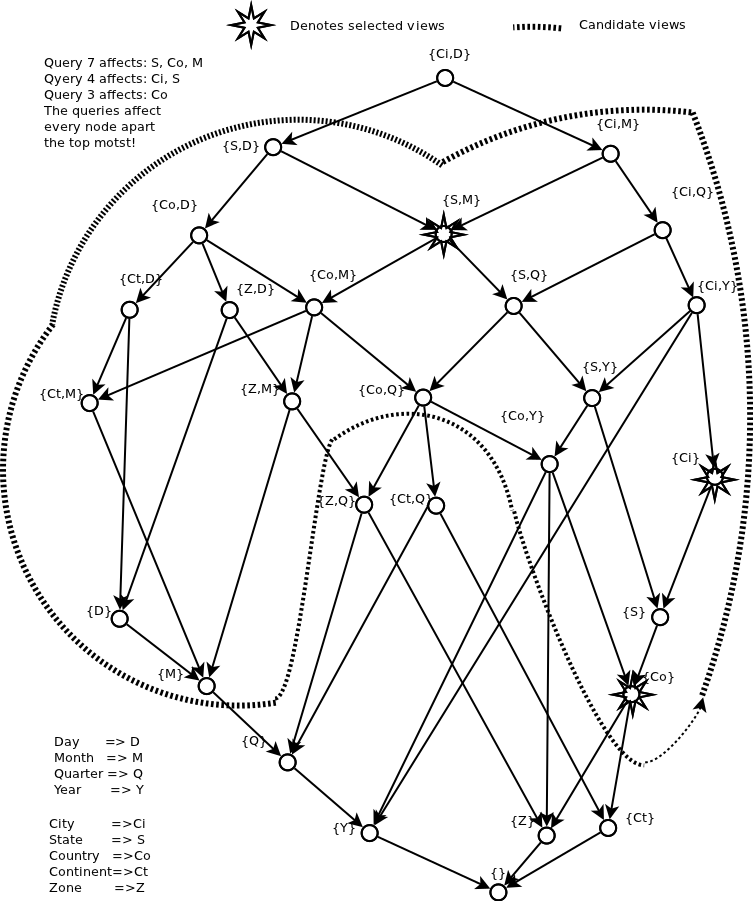
\includegraphics[scale=0.45]{lattice}
\caption{\label{fig:lattice}  Lattice}
\end{center}
\end{figure}


